\begin{figure}[htbp]
\centering
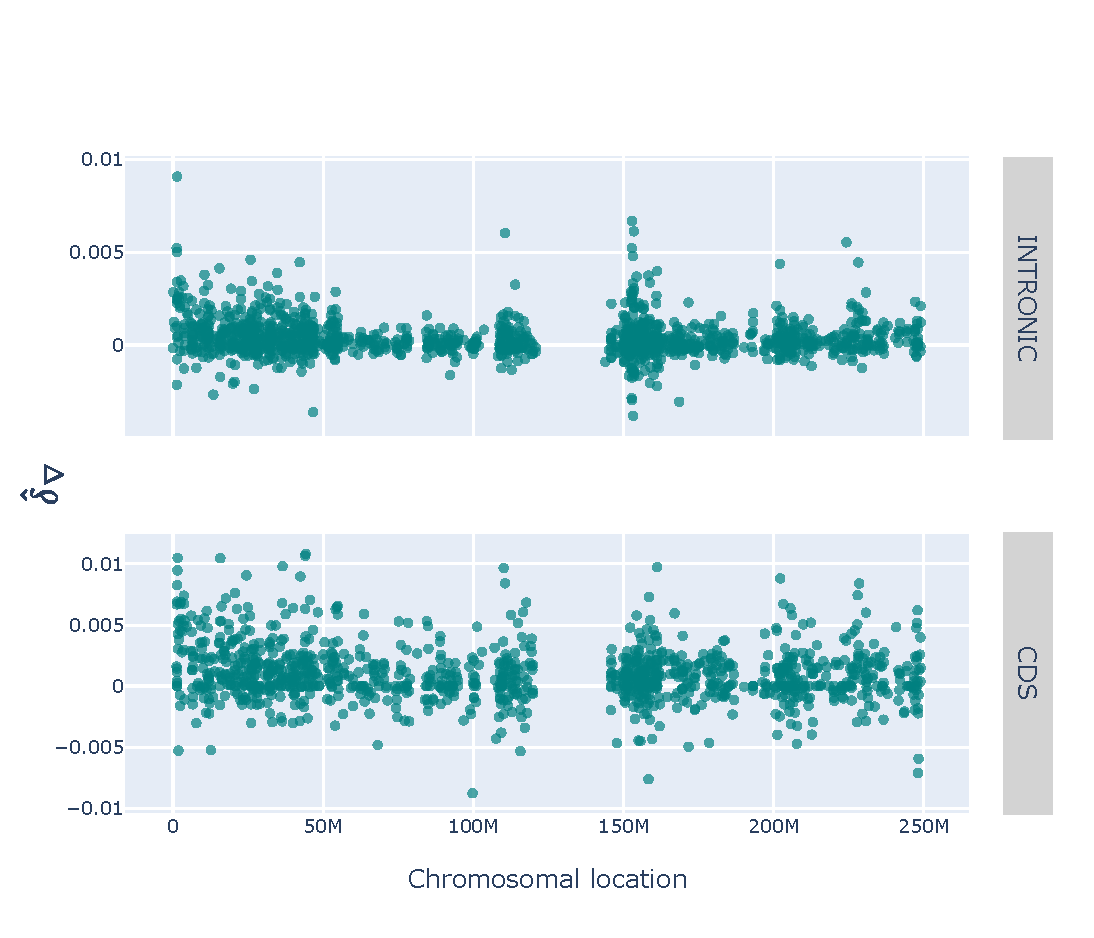
\includegraphics[width=	\textwidth]{figures/plots/primate/d-conv-manhatten.pdf}
\caption{\textbf{The magnitude of disequilibrium is heterogeneous along a chromosome.} Manhattan plots show the position of a gene in a chromosome and the $\hat\delta_\nabla$ for the intronic (top) and CDS sequence (bottom) of that gene. Intronic data included 1,406 alignments CDS data included 1,182. The taxa in all alignments were human, chimpanzee and gorilla, in all model fitting human was the foreground edge. }
\label{fig:primate:dconv-manhattan}
\end{figure}
